%%%%%%%%%%%%%%%%%%%%%%%%%%%%%%%%%%%%%%%%%%%%%%%%%%%%%%%%%%%%%%%%%%%%%%%%%%%%%%%%
\section{Databases And Capture Methods}\label{ch:bg_db_capture}
%%%%%%%%%%%%%%%%%%%%%%%%%%%%%%%%%%%%%%%%%%%%%%%%%%%%%%%%%%%%%%%%%%%%%%%%%%%%%%%%
In contrast to generic shape recovery, facial shape recovery implies a strong
assumption that the input image contains a face. This prior knowledge, that the
image contains a face, enables the use of training data to improve the
quality of the reconstruction. \cref{tbl:timeline_db} provides a
timeline outlining the existing 3D facial databases and the data they provide.
It is particularly interesting to note that, despite the fact that one of the
first 3D facial models was released in 1987 (CANDIDE~\cite{Rydfalk:1987tg}), the
majority of existing databases were produced in the last decade. The quality
of these facial models has also increased substantially. 

The CANDIDE~\cite{Rydfalk:1987tg,Ahlberg:1998uk} models were parametrizable
wireframe models that contained a low number of vertices (75--95) and were
designed to be controlled according to pre-defined Action Units. The CANDIDE
model was not captured from real data and thus had limited uses for modelling
identity. Early attempts at recording facial databases focused on the use
of laser scanning technology~\cite{cyberware,minolta} or structured light. For
example, the early work of \citep{beumier2001face} used an internally developed 
structured light system to provide low quality neutral face scans. Structured
light was also used for the Bosphorus~\cite{Savran:2008gg} 
and UoY~\cite{heseltine2008three} databases. One of the most commonly used
parametric 3D models is that of the Basel 3D Morphable Model 
(3DMM)~\cite{paysan20093d} which also utilized a custom structured light
scanner called the ABW-3D scanner. The introduction of the consumer priced
Kinect by Microsoft ensured that structured light technology was extremely 
cheap to acquire and thus both the BIWI Head Pose~\cite{fanelli2013random}, 
EURECOM~\cite{min2014kinectfacedb} and the FaceWarehouse~\cite{Cao:2014gy} 
databases used the Kinect for capturing data.

Researchers at the MPI used the \citet{cyberware} laser scanner to capture
neutral faces of high quality which were used in the seminal work of the 3DMM
by \citet{RefWorks:96}. The Cyberware scanner was also employed in the more 
recent works of BJUT-3D~\cite{baocai2009bjut} and Beckmann~\cite{hu2007building}
as it provides high quality shape and texture. Another commonly used
laser scanning system is the Minolta Vivid 900/910~\cite{minolta} which was
employed by Notre Dame University when collecting data for the Facial
Recognition Grand Challenge (FRGC)~\cite{phillips2005overview} and the following
ND-2006~\cite{faltemier2007using}. It was also employed by Notre Dame for the
collection of a twins database (3D-TEC)~\cite{vijayan2011twins}. 
The Konika Minolta was also for the databases of CASIA 3D~\cite{casia3d},
FSU~\cite{hesher2003novel} and the UMB-DB~\cite{colombo2011umb} which is unique
in containing many examples of occlusions. The more advanced
Minolta VI-700 digitizer~\cite{minolta} was used to collect both
GavabDB~\cite{moreno2004gavabdb} and FRAV3D~\cite{conde2006multimodal}.
ZJU-3DFED~\cite{wang2006exploring} used a white-light digitizer to capture
the 40 subjects of their work. 

Stereo systems provide a non-invasive method of capturing that is possible
to set up at relatively low cost by an expert. One of the earliest databases
to provide 3D face estimates was XM2VTSdb~\cite{messer1999xm2vtsdb}. 
Commercial systems such as
the 3dMD scanning system~\cite{3dmd} have been used by the 
BU3D-FE~\cite{Yin:2006cc} and the very recent 3DMM provided by 
Surrey University~\cite{Huber:F5Dca9zy}. A similar stereo capture
system was was for the Texas 3DFRD~\cite{gupta2010anthropometric} database.
Other than the Kinect,
which provides extremely low quality depth estimates, capturing high-quality 4D
(3D video) data has only been possible by performing stereo reconstructions from
multiple calibrated cameras. For example, the commercial system of \citet{di4d}
is capable of capturing high resolution images and converting them into
3D meshes at 60 FPS. The Di4D~\cite{di4d} scanning system has been used for
the only publicly available 4D databases of BU4D-FE~\cite{yin2008high} and
BP4D-Spontaneous~\cite{Zhang:2014id}. BP4D-Spontaneous is unique in that it
contains spontaneously produced emotions rather than the posed expressions
that are more common in other existing databases. A custom system combining
stereo and active light was used by the 
B3D (AC)\textsuperscript{2}~\cite{weise2007fast,fanelli2013random} database to
provide 17 FPS scanning of faces.

There have also been efforts to collect databases using illumination constraints
whereby 3D shape is generally recovered using Photometric Stereo (PS) 
algorithms. One of the earliest examples of such a database is the 
YaleB~\cite{RefWorks:314} database which contains 10 subjects captured in 
9 poses each under 64 illumination conditions. A large scale PS database was
provided by the Photoface database~\cite{RefWorks:293} which provided a low-cost
and practical methodology for capturing illuminated images in a public setting.
The ICT-3DRFE~\cite{stratou2012exploring} database provides multiple expressions
of 23 subjects captured by a 156 light ``light-stage''. Millimetre-accurate
facial shape is recovered through computational stereo and high frequency 
mesoscopic detail is recovered via the spherical lighting conditions proposed
by \citet{ma2007rapid}. The ICT-3DRFE database thus provides a dense 
3D facial mesh, as well as a diffuse and specular texture map and diffuse and
specular normals.

The majority of the databases above were collected using commercial apparatus
and the focus of the database was the gathering of the subjects rather than the
capturing methodology itself. However, the capturing of high quality facial
surface information is an active area of research and is of particular interest
to the computer graphics community. High quality facial surface information
including high frequency mesoscopic details such as fine wrinkles and pores is
required for photo-realistic rendering of faces and has applications in
films~\cite{borshukov2005universal}, video games~\cite{vonderPahlen:2014kg},
virtual makeup systems~\cite{scherbaum2011computer} and
animatronics~\cite{jung2011believable}. The recover of these mesoscopic details
requires careful modelling of the interaction between light and human skin. To
this end, many works focus solely on these reflectance characteristics and seek
to provide highly realistic parametric reflectance functions for human skin. In
this review, we are only interested in methods that recover realistic 3D shape
and thus do not consider works that focus solely on reflectance function
modelling. The interested reader should consult the recent survey on facial
appearance capture by \citet{Klehm:2015jb}. The state-of-the-art methods
for 3D facial capture 
%%%%%%%%%%%%%%%%%%%%%%%%%%%%%%%%%%%%%%%%
\begin{figure}[t]
	\centering
	\begin{subfigure}[b]{0.18\textwidth}
		\centering
		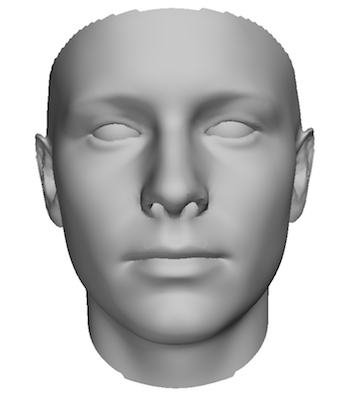
\includegraphics[height=1.5in]{background/images/basel}
		\caption{Basel}\label{fig:db_examples_basel}
	\end{subfigure}
	\begin{subfigure}[b]{0.18\textwidth}
		\centering
		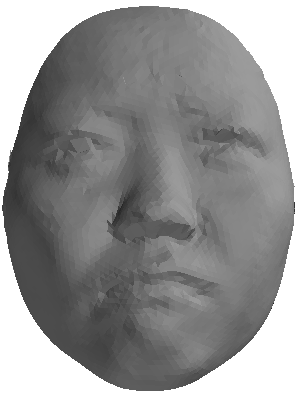
\includegraphics[height=1.7in]{background/images/bu3d}
		\caption{BU3D-FE}\label{fig:db_examples_bu3d}
	\end{subfigure}
	\begin{subfigure}[b]{0.18\textwidth}
		\centering
		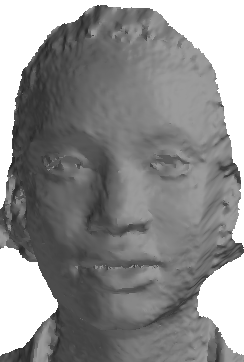
\includegraphics[height=1.7in]{background/images/bp4d}
		\caption{BP4D-S}\label{fig:db_examples_bp4d}
	\end{subfigure}
	\begin{subfigure}[b]{0.18\textwidth}
		\centering
		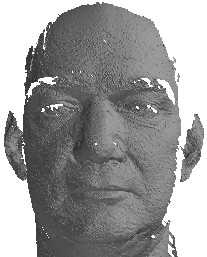
\includegraphics[height=1.7in]{background/images/frgc}
		\caption{FRGC v2}\label{fig:db_examples_frgc}
	\end{subfigure}
	\begin{subfigure}[b]{0.18\textwidth}
		\centering
		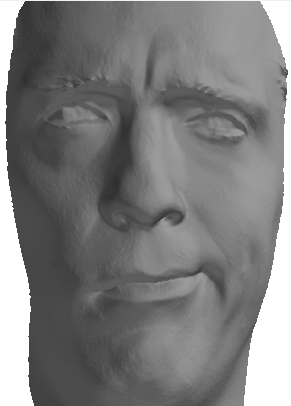
\includegraphics[height=1.7in]{background/images/ict}
		\caption{ICT-3DRFE}\label{fig:db_examples_ict}
	\end{subfigure}
	\caption{Examples of the quality of the facial meshes provided in various
	         databases.}
\label{fig:db_examples}
\end{figure}
%%%%%%%%%%%%%%%%%%%%%%%%%%%%%%%%%%%%%%%%
%%%%%%%%%%%%%%%%%%%%%%%%%%%%%%%%%%%%%%%%
% CANDIDE 3d wireframe model
% MPI     7 views, 200 laser scanned heads, 5 full 3D, Cyberware, static, neutral
% ND-D    953 scans, Minolta Vivid 900 3D scanner, 656 subjects, neutral, static
% ND-2006 13,450 images containing 6 different types of expressions, 888 distinct people
%         Static, Minolta Vivid 910 range scanner
% 3D-TEC 212 individuals (106 twins),  Minolta VIVID 910 3D scanner, 1 neutral, 1 smiling, static
% CASIA 3D 4624 scans of 123 persons, Minolta Vivid 910, various poses, emotions, static
% B3D(AC)^2 scanned using \cite{weise2007fast}, 14 subjects, 1109 sequences, dynamic 25 FPS, reading
% BIWI Head Pose  15K images of 20 people, various head poses, missing frames, kinect
% UOY Face Database 97 people, multi-pose, neutral, smile and frown
% GavabDB 61 individuals, 427 images, multi pose, static, 3 expressions
% FRAV3D 106 subjects,  MINOLTA VIVID-700, multi-pose, static
% Basel 200 scans, neutral, ABW-3D structured light scanner
% BJUT-3D, cyberware
% EURECOM Kinect, 52 people * 18 image, multi poses, expressions, static
% XM2VTS stereo, 25 subjects, neutral,
% Texas 3DFRD 1149 pairs of facial color and range images of 105 adult human subjects,
%             stereo imaging system manufactured by 3Q Technologies, neutral, frontal
% ZJU-3DFED  40 subjects, total 360, expressions, InSpeck 3D MEGA Capturor DF
% 3D_RMA structured light, 120 people, 6 shots, multi-pose
% Beckmann cyberware, 400-500, single shot
% UMB-DB Minolta Vivid 900 laser scanner
\begin{table}[h]
\centering
\resizebox{\textwidth}{!}{%
\begin{tabular}{@{}cccccccc@{}}
\toprule
\multicolumn{3}{c}{DB}                                                              & \# Subjects & \# Outputs  & Expressions  & Poses        & Type   \\ \midrule
CANDIDE v1                  &\cite{Rydfalk:1987tg}          & 1987                  & 1           & 1           & $\checkmark$ & ---          & MO     \\ \midrule
MPI                         &\cite{Troje:1996ep}            & 1996                  & 200         & 200         &              &              & M      \\ \midrule
CANDIDE v2                  &\cite{Ahlberg:1998uk}          & \multirow{2}{*}{1998} & 1           & 1           & $\checkmark$ & ---          & MO     \\
3D\_RMA                     &\cite{beumier2001face}         &                       & 120         & 720         &              & $\checkmark$ & D      \\ \midrule
USF                         &\cite{RefWorks:96}             & \multirow{3}{*}{1999} & 200         & 200         &              & ---          & MO     \\
XM2VTSdb                    &\cite{messer1999xm2vtsdb}      &                       & 295         & 2360        &              &              & M      \\
YaleB                       &\cite{RefWorks:314}            &                       & 10          & 5760        & $\checkmark$ &              & PS     \\ \midrule
CASIA 3D                    &\cite{casia3d}                 & \multirow{2}{*}{2003} & 123         & 1845        & $\checkmark$ &              & D      \\
FSU                         &\cite{hesher2003novel}         &                       & 37          & 222         & $\checkmark$ &              & D      \\ \midrule
GavabDB                     &\cite{moreno2004gavabdb}       & 2004                  & 61          & 720         & $\checkmark$ & $\checkmark$ & D      \\ \midrule
FRGC v2                     &\cite{phillips2005overview}    & 2005                  & 466         & 4007        & $\checkmark$ &              & D      \\ \midrule
BU3D-FE                     &\cite{Yin:2006cc}              & \multirow{4}{*}{2006} & 100         & 2500        & $\checkmark$ &              & M      \\
ND-2006                     &\cite{faltemier2007using}      &                       & 888         & 13450       & $\checkmark$ &              & D      \\
FRAV3D                      &\cite{conde2006multimodal}     &                       & 106         & 1696        & $\checkmark$ &              & M      \\
ZJU-3DFED                   &\cite{wang2006exploring}       &                       & 40          & 360         & $\checkmark$ &              & M      \\ \midrule
Beckmann                    &\cite{hu2007building}          & 2007                  & $\sim$400   &~?           & $\checkmark$ &              & M      \\ \midrule
Bosphorus                   &\cite{Savran:2008gg}           & \multirow{3}{*}{2008} & 105         & 4652        & $\checkmark$ &              & M      \\
UoY                         &\cite{heseltine2008three}      &                       & 350         & 5250        & $\checkmark$ & $\checkmark$ & M      \\
BU4D-FE                     &\cite{yin2008high}             &                       & 101         & Many        & $\checkmark$ & $\checkmark$ & 4D M   \\ \midrule
Basel                       &\cite{paysan20093d}            & \multirow{2}{*}{2009} & 200         & 200         &              & ---          & MO     \\
BJUT-3D                     &\cite{baocai2009bjut}          &                       & 500         & 500         &              &              & M      \\ \midrule
B3D (AC)\textsuperscript{2} &\cite{fanelli20103}            & \multirow{2}{*}{2010} & 14          & Many        & $\checkmark$ &              & 4D D/M \\
Texas 3DFRD                 &\cite{gupta2010anthropometric} &                       & 118         & 1149        &              &              & M      \\ \midrule
3D-TEC                      &\cite{vijayan2011twins}        & \multirow{3}{*}{2011} & 212         & 212         & $\checkmark$ &              & M      \\
BIWI Head Pose              &\cite{fanelli2013random}       &                       & 20          & $\sim$15000 &              & $\checkmark$ & D      \\
UMB-DB                      &\cite{colombo2011umb}          &                       & 143         & 1473        & $\checkmark$ &              & M      \\ \midrule
ICT-3DRFE                   &\cite{stratou2012exploring}    & 2012                  & 23          & 345         & $\checkmark$ &              & PS     \\ \midrule
Photoface                   &\cite{RefWorks:293}            & 2013                  & 261         & 1839        & $\checkmark$ &              & PS/M   \\ \midrule
FaceWarehouse               &\cite{Cao:2014gy}              & \multirow{3}{*}{2014} & 150         & 3000        & $\checkmark$ & ---          & MO/D   \\
BP4D-Spontaneous            &\cite{Zhang:2014id}            &                       & 41          & Many        & $\checkmark$ & $\checkmark$ & 4D M   \\
EURECOM                     &\cite{min2014kinectfacedb}     &                       & 52          & 936         & $\checkmark$ & $\checkmark$ & D      \\ \midrule
SURREY                      &\cite{Huber:F5Dca9zy}          & 2016                  & 169         & 169         &              & ---          & MO     \\ \bottomrule
\end{tabular}%
}
\caption{A timeline of existing 3D facial databases including depth data, mesh
         data, models and Photometric Stereo images. PS denotes Photometric
         Stereo images, MO is a statistical model, M is a 3D mesh, 
         D is depth/range data and 4D implies a 3D video.}
\label{tbl:timeline_db}
\end{table}
%%%%%%%%%%%%%%%%%%%%%%%%%%%%%%%%%%%%%%%%
%%%%%%%%%%%%%%%%%%%%%%%%%%%%%%%%%%%%%%%%%%%%%%%%%%%%%%%%%%%%%%%%%%%%%%%%%%%%%%%%
